\documentclass[14pt]{beamer}
\usetheme{EastLansing}
\usecolortheme{spruce}

\usepackage{xcolor}
\usepackage{listings}
\usepackage{courier}
\usepackage{graphicx}
\usepackage{amsmath}
\usepackage{algorithm2e}
\usepackage{multicol}

% https://tex.stackexchange.com/questions/42619/x-mark-to-match-checkmark
\usepackage{pifont}% http://ctan.org/pkg/pifont

%% https://stackoverflow.com/questions/1435837/how-to-remove-footers-of-latex-beamer-templates
%%gets rid of bottom navigation bars
%\setbeamertemplate{footline}[page number]
%
%gets rid of navigation symbols
\setbeamertemplate{navigation symbols}{}


\usefonttheme[onlymath]{serif}

\definecolor{mGreen}{rgb}{0,0.6,0}
\definecolor{mGray}{rgb}{0.5,0.5,0.5}
\definecolor{mPurple}{rgb}{0.8,0,0.82}
\definecolor{backgroundColour}{rgb}{0.95,0.95,0.92}
\definecolor{lightBlue}{rgb}{0.1, 0.1, 0.8}

\newcommand\red[1]{{\color{red} #1}}
\newcommand\green[1]{{\color{green} #1}}
\newcommand\blue[1]{{\color{blue} #1}}

\newcommand{\cmark}{\ding{51}}%
\newcommand{\xmark}{\ding{55}}%

\lstdefinestyle{CStyle}{
    backgroundcolor=\color{backgroundColour},   
    commentstyle=\color{mGreen},
    keywordstyle=\color{magenta},
    numberstyle=\tiny\color{mGray},
    stringstyle=\color{mPurple},
    basicstyle=\footnotesize,
    breakatwhitespace=false,         
    breaklines=true,                 
    captionpos=b,                    
    keepspaces=true,                 
    numbers=left,                    
    numbersep=5pt,                  
    showspaces=false,                
    showstringspaces=false,
    showtabs=false,                  
    tabsize=2,
    language=C
}
\lstdefinestyle{pseudo}{
        basicstyle=\ttfamily\footnotesize,
        keywordstyle=\color{lightBlue},
        morekeywords={BEGIN,END,IF,ELSE,ENDIF,ELSEIF,PRINT,WHILE,RETURN,ENDWHILE,DO,FOR,TO,IN,ENDFOR,BREAK,INPUT},
        morecomment=[l]{//},
        commentstyle=\color{mGreen}
}

\lstset{basicstyle=\footnotesize\ttfamily,breaklines=true}
\lstset{framextopmargin=50pt,tabsize=2}

\title{ENGG1003 - Thursday Week 2}
\subtitle{Data types, and introduction to arrays}
\author{Steve Weller}
\institute{University of Newcastle}
%\date{\today}
\date{4 March, 2021}

% following is a bit of a hack, but forces page numbers (technically: frame numbers) to run 1,2,3,... 
% with titlepage counting as frame 1

\addtocounter{framenumber}{1}
\titlepage

\begin{document}
\framebreak

%==============================================================

\begin{frame}[fragile]

\frametitle{Lecture overview}
\begin{enumerate}
	\item variables and data types \red{\S2.2}
	\begin{itemize}
		\item principles
		\item live demo
	\end{itemize}

	\item[]
	
	\item arrays in Python \red{\S2.3}
		\begin{itemize}
			\item principles
			\item live demo
		\end{itemize}

\end{enumerate}

\end{frame}

%\begin{itemize}
%	\item xxx
%\end{itemize}

%==============================================================

\begin{frame}[fragile]

\frametitle{$1)$ variables and data types}

\begin{itemize}
	\item variable names---make them descriptive but short(-ish), not always easy!
		\begin{itemize}
			\item[\green{\cmark}]  waterLevel, altitudeUAV, tunnelDepth
			\item[\red{\xmark}] w, a, t
			\item[\red{\xmark}] averageAnnualBatteryVoltage
		\end{itemize}
	\item camelCase
		\begin{itemize}
			\item lower camel case eg: iPhone, macOS
			\item upper camel case eg: PlayStation, YouTube
		\end{itemize}
	\item snake$\_$case
		\begin{itemize}
			\item also known as lower\_case\_with\_underscores
		\end{itemize}
	\item matter of preference/style/taste
		\begin{itemize}
			\item experiment, find what works best for you! %, won't be marked down for ``wrong'' style!			
		\end{itemize}
\end{itemize}

\end{frame}

%==============================================================

\begin{frame}[fragile]

\frametitle{Assignment}

\begin{itemize}
	\item \texttt{x = 2}
	\begin{itemize}
		\item ``variable \texttt{x} is assigned the value of $2$''
	\end{itemize}
	\item[]
	\item \texttt{x = x + 4}
	\begin{itemize}
		\item value of \texttt{x} is increased by $4$
		\item new value of \texttt{x} over-writes old value
	\end{itemize}
	\item[]
	\item abbreviations
		\begin{itemize}
		\item \texttt{x+= 4} is short for \texttt{x = x + 4}
		\item \texttt{x -= 4} $\Longleftrightarrow$  \texttt{x = x - 4}
		\item \texttt{x *= 4} $\Longleftrightarrow$ \texttt{x = x * 4}
		\item \texttt{x /= 4} $\Longleftrightarrow$ \texttt{x = x / 4}
	\end{itemize}

\end{itemize}

\end{frame}

%==============================================================

\begin{frame}[fragile]

\frametitle{Data types in Python}

Python data types of variables seen so far:

	\begin{itemize}
		\item \textbf{\texttt{int}}
		\item \textbf{\texttt{float}}
		\item \textbf{\texttt{str}}
		\item one more data type will be introduced next week *dramatic music plays*
	\end{itemize}
	
\begin{itemize}
\item[]
	\begin{itemize}
		\item \texttt{int}---integers, eg: $0,1,9,-10,452617$
		\item \texttt{float}---real numbers, eg: $3.14159, -5.5, 2.0$
			\begin{itemize}
				\item will explain ``floating point number'' terminology later
			\end{itemize}
		\item \texttt{str}---strings, eg: `Hello ENGG1003'
	\end{itemize}
%	\item mention ``objects'' only in passing
\end{itemize}

\end{frame}

%%==============================================================
%
%\begin{frame}[fragile]
%
%\frametitle{The type of a variable (ctd.)}
%
%\end{frame}

%==============================================================

\begin{frame}[fragile]

\frametitle{Type function}

\begin{itemize}
	\item \red{\S2.2.4} and \red{\S2.2.5}
	\item built-in function \texttt{type}
	\item type conversion
	\item automatic type conversion
\end{itemize}

\end{frame}

%%==============================================================
%
%\begin{frame}[fragile]
%
%\frametitle{Operator precedence---OMIT??}
%
%\end{frame}
%
%%==============================================================
%
%\begin{frame}[fragile]
%
%\frametitle{Division---quotient and remainder---OMIT??}
%
%\end{frame}

%==============================================================

\begin{frame}[fragile]
\frametitle{Live demo of variables and data types}

\end{frame}

%==============================================================

\begin{frame}[fragile]

\frametitle{2) Arrays in Python}

\begin{itemize}
	\item simple arrays appeared in Monday's lecture
	\begin{itemize}
		\item height of a ball was computed for each millisecond
		\item time stored in array \texttt{t}
		\item height stored in array \texttt{y}
	\end{itemize}
	\item[]
	\item arrays we use in this course are imported from \texttt{numpy} library
	\item[]
	\item for each array, all array \red{\emph{elements}} must be of the same type
	\begin{itemize}
		\item eg: all \texttt{int}, or all \texttt{float}
	\end{itemize}
		
\end{itemize}

\end{frame}

%==============================================================

\begin{frame}[fragile]

\frametitle{Array creation and array elements}

	\begin{figure}[ht]
		\centering
		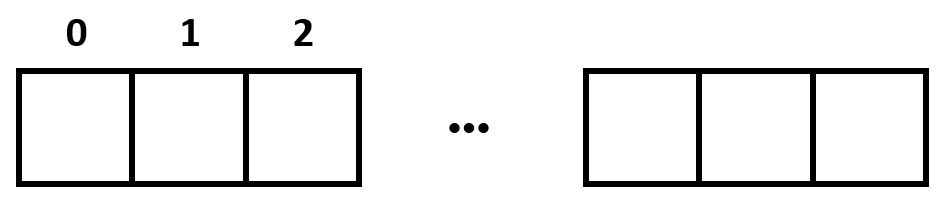
\includegraphics[width=0.6\textwidth]{figures/arrayElements012}
	\end{figure}

\vspace*{-4mm}

\begin{itemize}

	\item array \red{\emph{index}} used to identify array elements
		\begin{itemize}
			\item Python uses \red{\emph{zero-based indexing}}
			\item indices start at zero: $0,1,2, \ldots$
%			\item plural: array \red{\emph{indices}}
		\end{itemize}
					
	\item[]
	\vspace*{-4mm}
							
	\item four common ways of creating arrays:
	\begin{itemize}
		\item \texttt{linspace}
		\item \texttt{zeros}
		\item \texttt{array}
		\item \texttt{copy}
	\end{itemize}
	
\end{itemize}

\end{frame}

%==============================================================

\begin{frame}[fragile]

\frametitle{\#1 Linspace}

\begin{itemize}
	\item have seen \texttt{linspace} function already
	\item \texttt{t = np.linspace(0, 1, 1001)} creates 1001 coordinates between 0 and 1, inclusive at both ends
	
	\begin{figure}[ht]
		\centering
		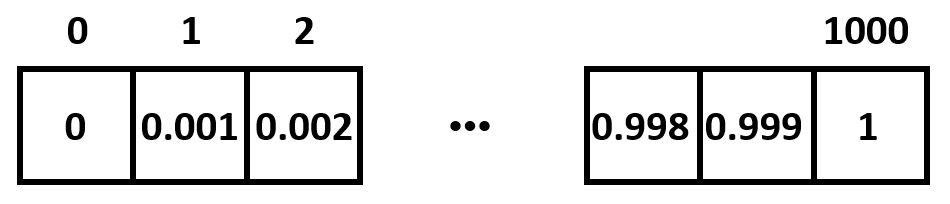
\includegraphics[width=0.6\textwidth]{figures/arrayElementsMilliseconds}
	\end{figure}

	\item \texttt{t} is the name of the array
	\item array indices are $0, 1, 2, \ldots$
	\item array elements:~\texttt{t[0]},~\texttt{t[1]},~\texttt{t[2]},~\ldots,~\texttt{t[1000]}
%	\item general form: if $n$ evenly spaced numbers are sought on interval $[a, b]$:
%	\item[]
%	\texttt{numpy.linspace(a, b, n)}
\end{itemize}

\end{frame}

%==============================================================

\begin{frame}[fragile]

\frametitle{}

\begin{figure}[ht]
	\centering
	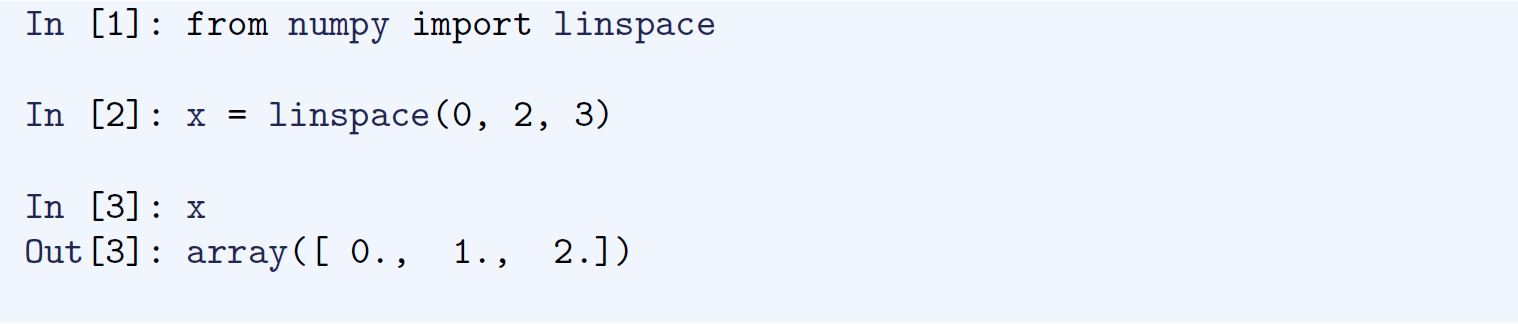
\includegraphics[width=\textwidth]{figures/LLp47}
	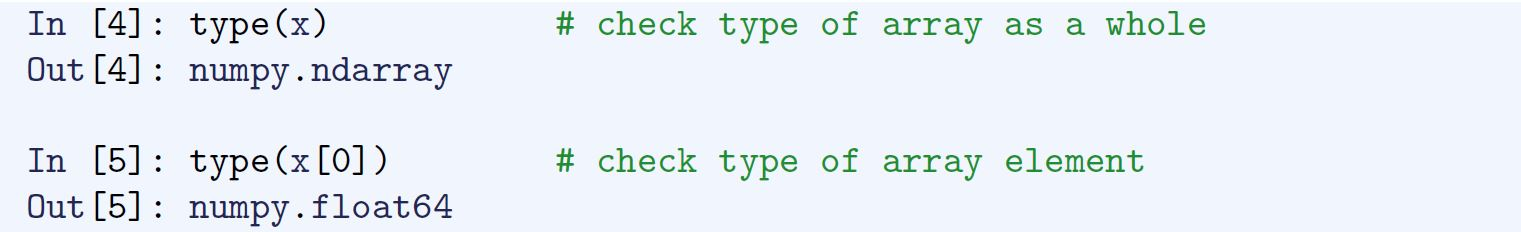
\includegraphics[width=\textwidth]{figures/LLp48}
\end{figure}

\vspace*{-4mm}
	
\begin{itemize}
	\item array has $3$ elements: \texttt{x[0], x[1], x[2]}
	\item individual array elements have type \texttt{numpy.float64}
	\begin{itemize}
		\item \texttt{float64} is a particular float data type in NumPy
	\end{itemize}
	\item array \texttt{x} itself has type \texttt{numpy.ndarray}

\end{itemize}

\end{frame}

%==============================================================

\begin{frame}[fragile]

\frametitle{\#2 Zeros function}

%\vspace*{-3mm}
\begin{figure}[ht]
	\centering
	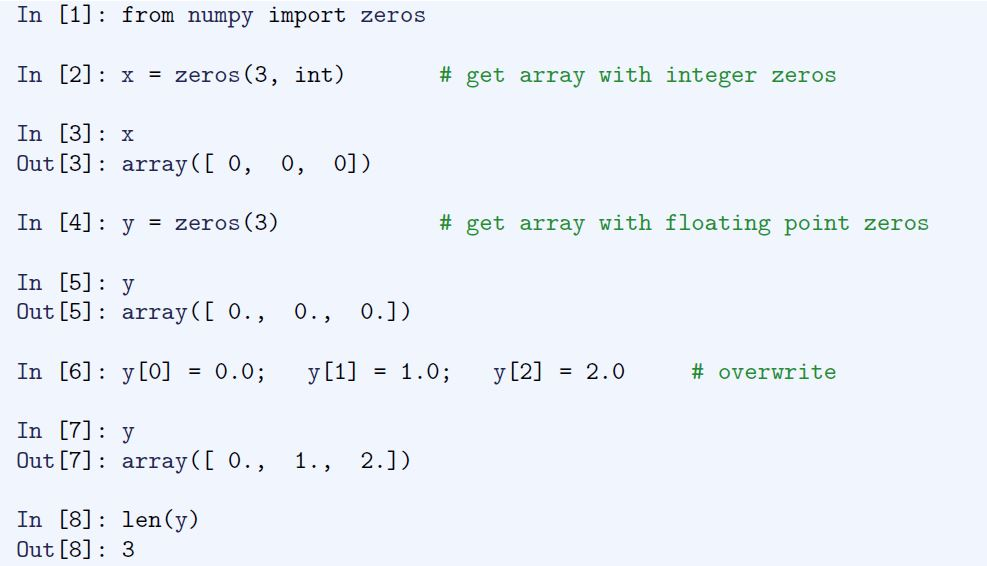
\includegraphics[width=\textwidth]{figures/LLp49}
\end{figure}

\end{frame}

%==============================================================

\begin{frame}[fragile]

\frametitle{}

\begin{itemize}
	\item array of \texttt{int} or array of \texttt{float}
	\begin{itemize}
		\item but cannot mix \texttt{int} and \texttt{float} type in one array!
	\end{itemize}
	\item \texttt{len(y)} is \red{\emph{length}} of array \texttt{y}
	\item zeros(3,int)
	\item zeros(3)
	\item 0 for int, 0. for float
\end{itemize}

\end{frame}

%==============================================================

\begin{frame}[fragile]

\frametitle{\#3 Array function}

\begin{itemize}
	\item create an array of zeros
	\item pp49-50 screenshot
	\item Note the use of ``dots'' to get floating point numbers
\end{itemize}

\end{frame}



%==============================================================

\begin{frame}[fragile]

\frametitle{Index out of bounds}

\begin{figure}[ht]
	\centering
	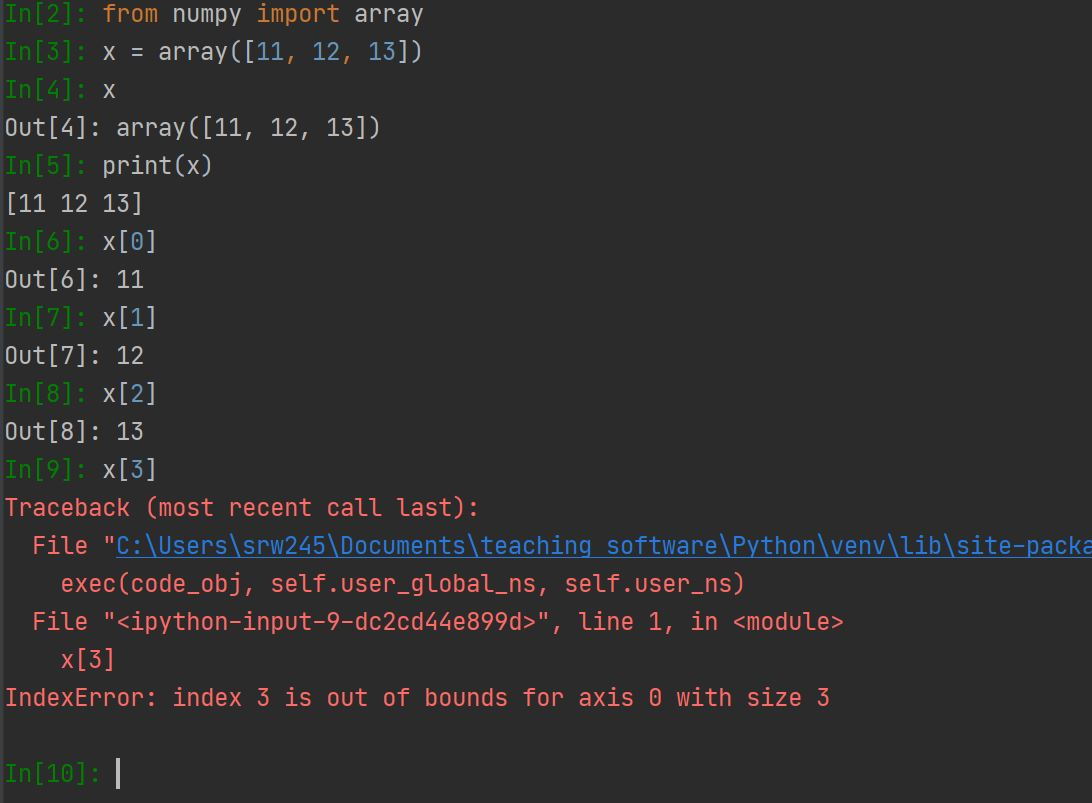
\includegraphics[width=0.6\textwidth]{figures/LLp50PyCharm}
\end{figure}
\vspace*{-5mm}
\begin{itemize}
	\item for array with 3 elements \texttt{x[0], x[1], x[2]}, only legal indices are $0,1$ and $2$
	\item ``out of bounds'' error if we try and access \texttt{x[3]}
%	\item contrast with C
\end{itemize}

\end{frame}

%==============================================================

\begin{frame}[fragile]

\frametitle{\#4 Copying an array---the problem}

\begin{itemize}
	\item \red{BE VERY CAREFUL} with naive/obvious copy method
	\item \texttt{copy} function creates new array and copies values
	\begin{itemize}
		\item use this method!
	\end{itemize}
\end{itemize}

\end{frame}

%==============================================================

\begin{frame}[fragile]

\frametitle{\#4 Copying an array---how to copy}

\begin{figure}[ht]
	\centering
	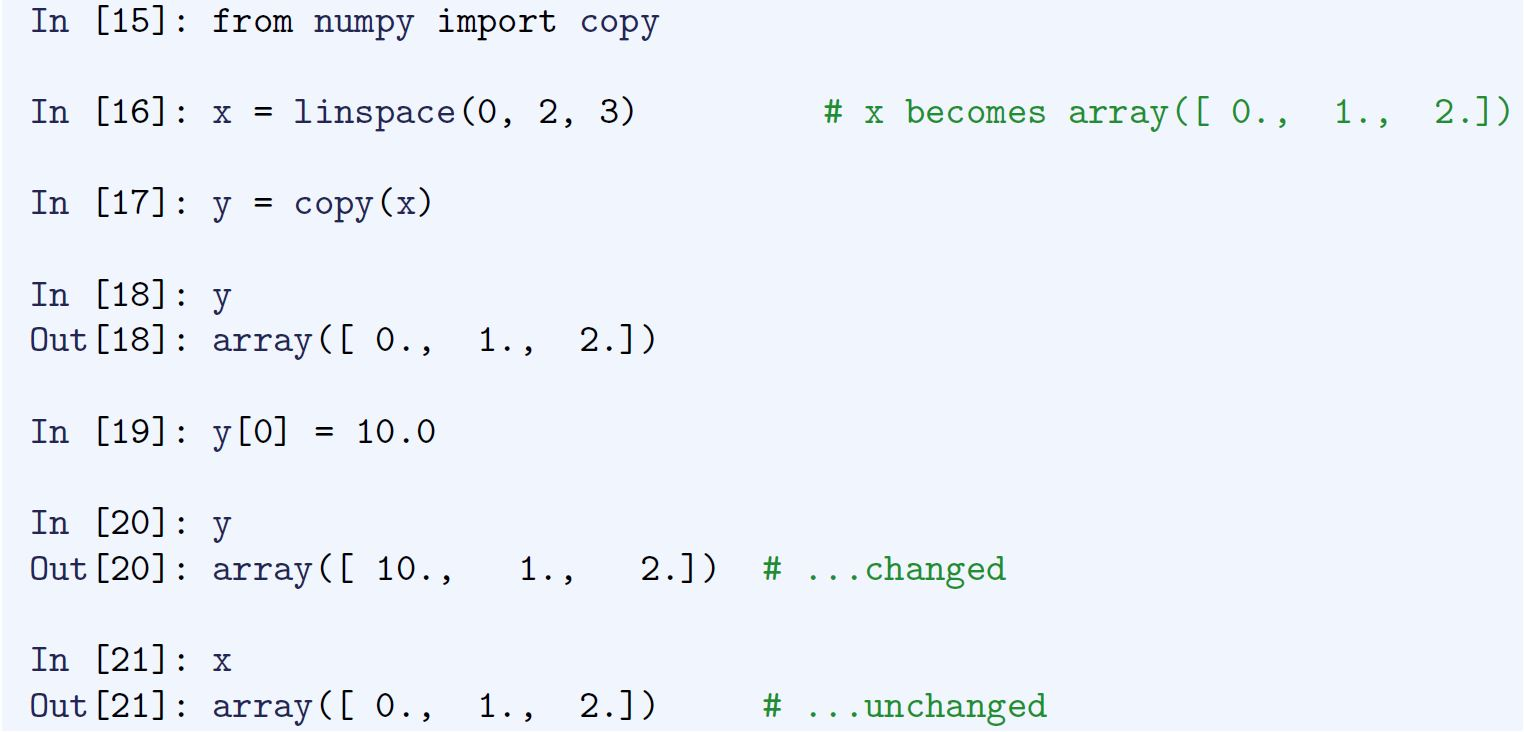
\includegraphics[width=0.9\textwidth]{figures/LLp51a}
\end{figure}

\vspace*{-5mm}

\begin{itemize}
	\item copy function--- actually \emph{creates} then copies values
\end{itemize}

\end{frame}

%==============================================================

\begin{frame}[fragile]

\frametitle{Slicing an array}

\begin{itemize}
	\item needs a figure showing boxes
	\item ppt figure
	\item colon x[i:j] address all elements from index i (inclusive) to j (exclusive)
		\begin{itemize}
			\item well that's confusing \ldots
		\end{itemize}
	\item x length 6, x[0],...x[5], write x[0:5], entries 11...16
	\item y length 5, subset x[1:5]  from y
	\item WARNING: When copying a slice, the same logic applies as when naively \emph{copying} the whole array
	\item no screenshot needed, but illustrate live (maybe)
\end{itemize}

\end{frame}

%==============================================================

\begin{frame}[fragile]

\frametitle{Slicing an array (ctd)}

\begin{figure}[ht]
	\centering
	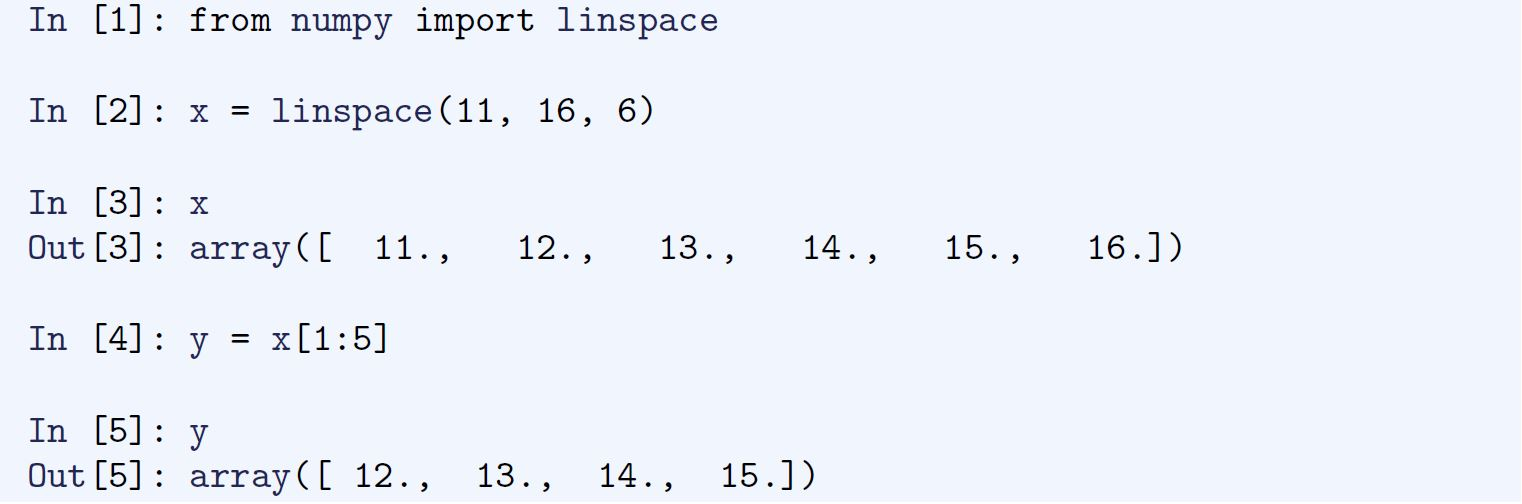
\includegraphics[width=\textwidth]{figures/LLp51}
\end{figure}

\end{frame}

%==============================================================

\begin{frame}[fragile]
\frametitle{Live demo of Python arrays}

\end{frame}

%%==============================================================
%
%\begin{frame}[fragile]
%
%\frametitle{}
%
%\end{frame}
%
%%==============================================================
%
%\begin{frame}[fragile]
%
%\frametitle{}
%
%\end{frame}
%
%%==============================================================
%
%\begin{frame}[fragile]
%
%\frametitle{}
%
%\end{frame}

\end{document}
